\section{SURF Surface Plot Function}

\subsection{Usage}

This routine is used to create a surface plot of data.  A 
surface plot is a 3D surface defined by the xyz coordinates
of its vertices and optionally by the color at the vertices.
The most general syntax for the \verb|surf| function is
\begin{verbatim}
  h = surf(X,Y,Z,C,properties...)
\end{verbatim}
Where \verb|X| is a matrix or vector of \verb|x| coordinates, \verb|Y| is a
matrix or vector of \verb|y| coordinates, \verb|Z| is a 2D matrix of
coordinates, and \verb|C| is a 2D matrix of color values (the colormap
for the current fig is applied).  In general, \verb|X| and \verb|Y| should
be the same size as \verb|Z|, but FreeMat will expand vectors to match
the matrix if possible.
If you want the color of the surface to be defined by the height
of the surface, you can omit \verb|C|
\begin{verbatim}
  h = surf(X,Y,Z,properties...)
\end{verbatim}
in which case \verb|C=Z|.  You can also eliminate the \verb|X| and \verb|Y|
matrices in the specification
\begin{verbatim}
  h = surf(Z,properties)
\end{verbatim}
in which case they are set to \verb|1:size(Z,2)| and \verb|1:size(Y,2)|
respectively.
You can also specify a handle as the target of the \verb|surf| command
via
\begin{verbatim}
  h = surf(handle,...)
\end{verbatim}
\subsection{Example}

Here we generate a surface specifying all four components.
@>


\centerline{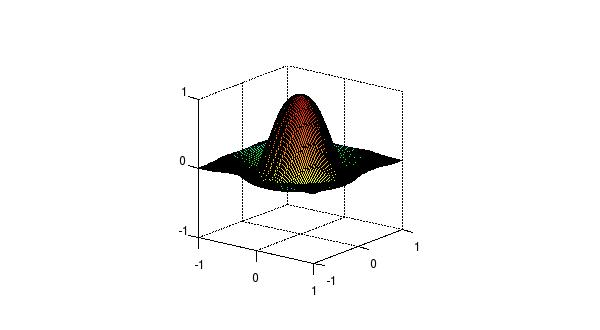
\includegraphics[width=8cm]{surf1}}

If we allow FreeMat to specify the color component, we see that
the colorfield is the same as the height
@>


\centerline{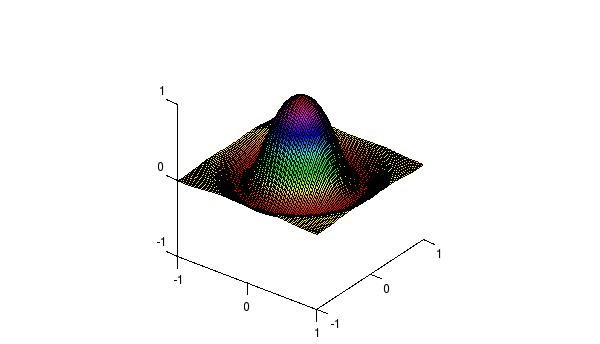
\includegraphics[width=8cm]{surf2}}

